Multi-scale transform (MST) theories are the most popular tools
used in various image fusion scenarios such as multi-focus image fusion, visible-infrared image fusion, and multimodal medical image fusion. Classical MST-based fusion methods include pyramid-based ones like Laplacian pyramid (LP)\cite{2} 
 ratio of low-pass pyramid (RP)\cite{3} and gradient pyramid (GP)\cite{4},wavelet-based ones like discrete wavelet transform (DWT)\cite{5},stationary wavelet transform (SWT) \cite{6} and dual-tree complex wavelet transform (DTCWT) \cite{7}, and multi-scale geometric analysis (MGA)-based ones like curvelet transform (CVT)\cite{8} and nonsubsampled contourlet transform (NSCT) \cite{9}. 
\hfill \break 
In the following section i am going to discuss some of above featured transformation.

\section{Laplacian pyramid Transformation}

Pyramid, or pyramid representation, is a type of multi-scale signal representation developed by the computer vision, image processing and signal processing communities, in which a signal or an image is subject to repeated smoothing and subsampling. Pyramid representation is a predecessor to scale-space representation and multiresolution analysis.

\subsection{Pyramid Generation}
There are two main types of pyramids: lowpass and bandpass.
\hfill \break
A lowpass pyramid is made by smoothing the image with an appropriate smoothing filter and then subsampling the smoothed image, usually by a factor of 2 along each coordinate direction. The resulting image is then subjected to the same procedure, and the cycle is repeated multiple times. Each cycle of this process results in a smaller image with increased smoothing, but with decreased spatial sampling density (that is, decreased image resolution). If illustrated graphically, the entire multi-scale representation will look like a pyramid, with the original image on the bottom and each cycle's resulting smaller image stacked one atop the other. \hfill \break

A bandpass pyramid is made by forming the difference between images at adjacent levels in the pyramid and performing some kind of image interpolation between adjacent levels of resolution, to enable computation of pixelwise differences.
\hfill \break
A variety of different smoothing kernels have been proposed for generating pyramids

\begin{figure}[h]
  \centering
  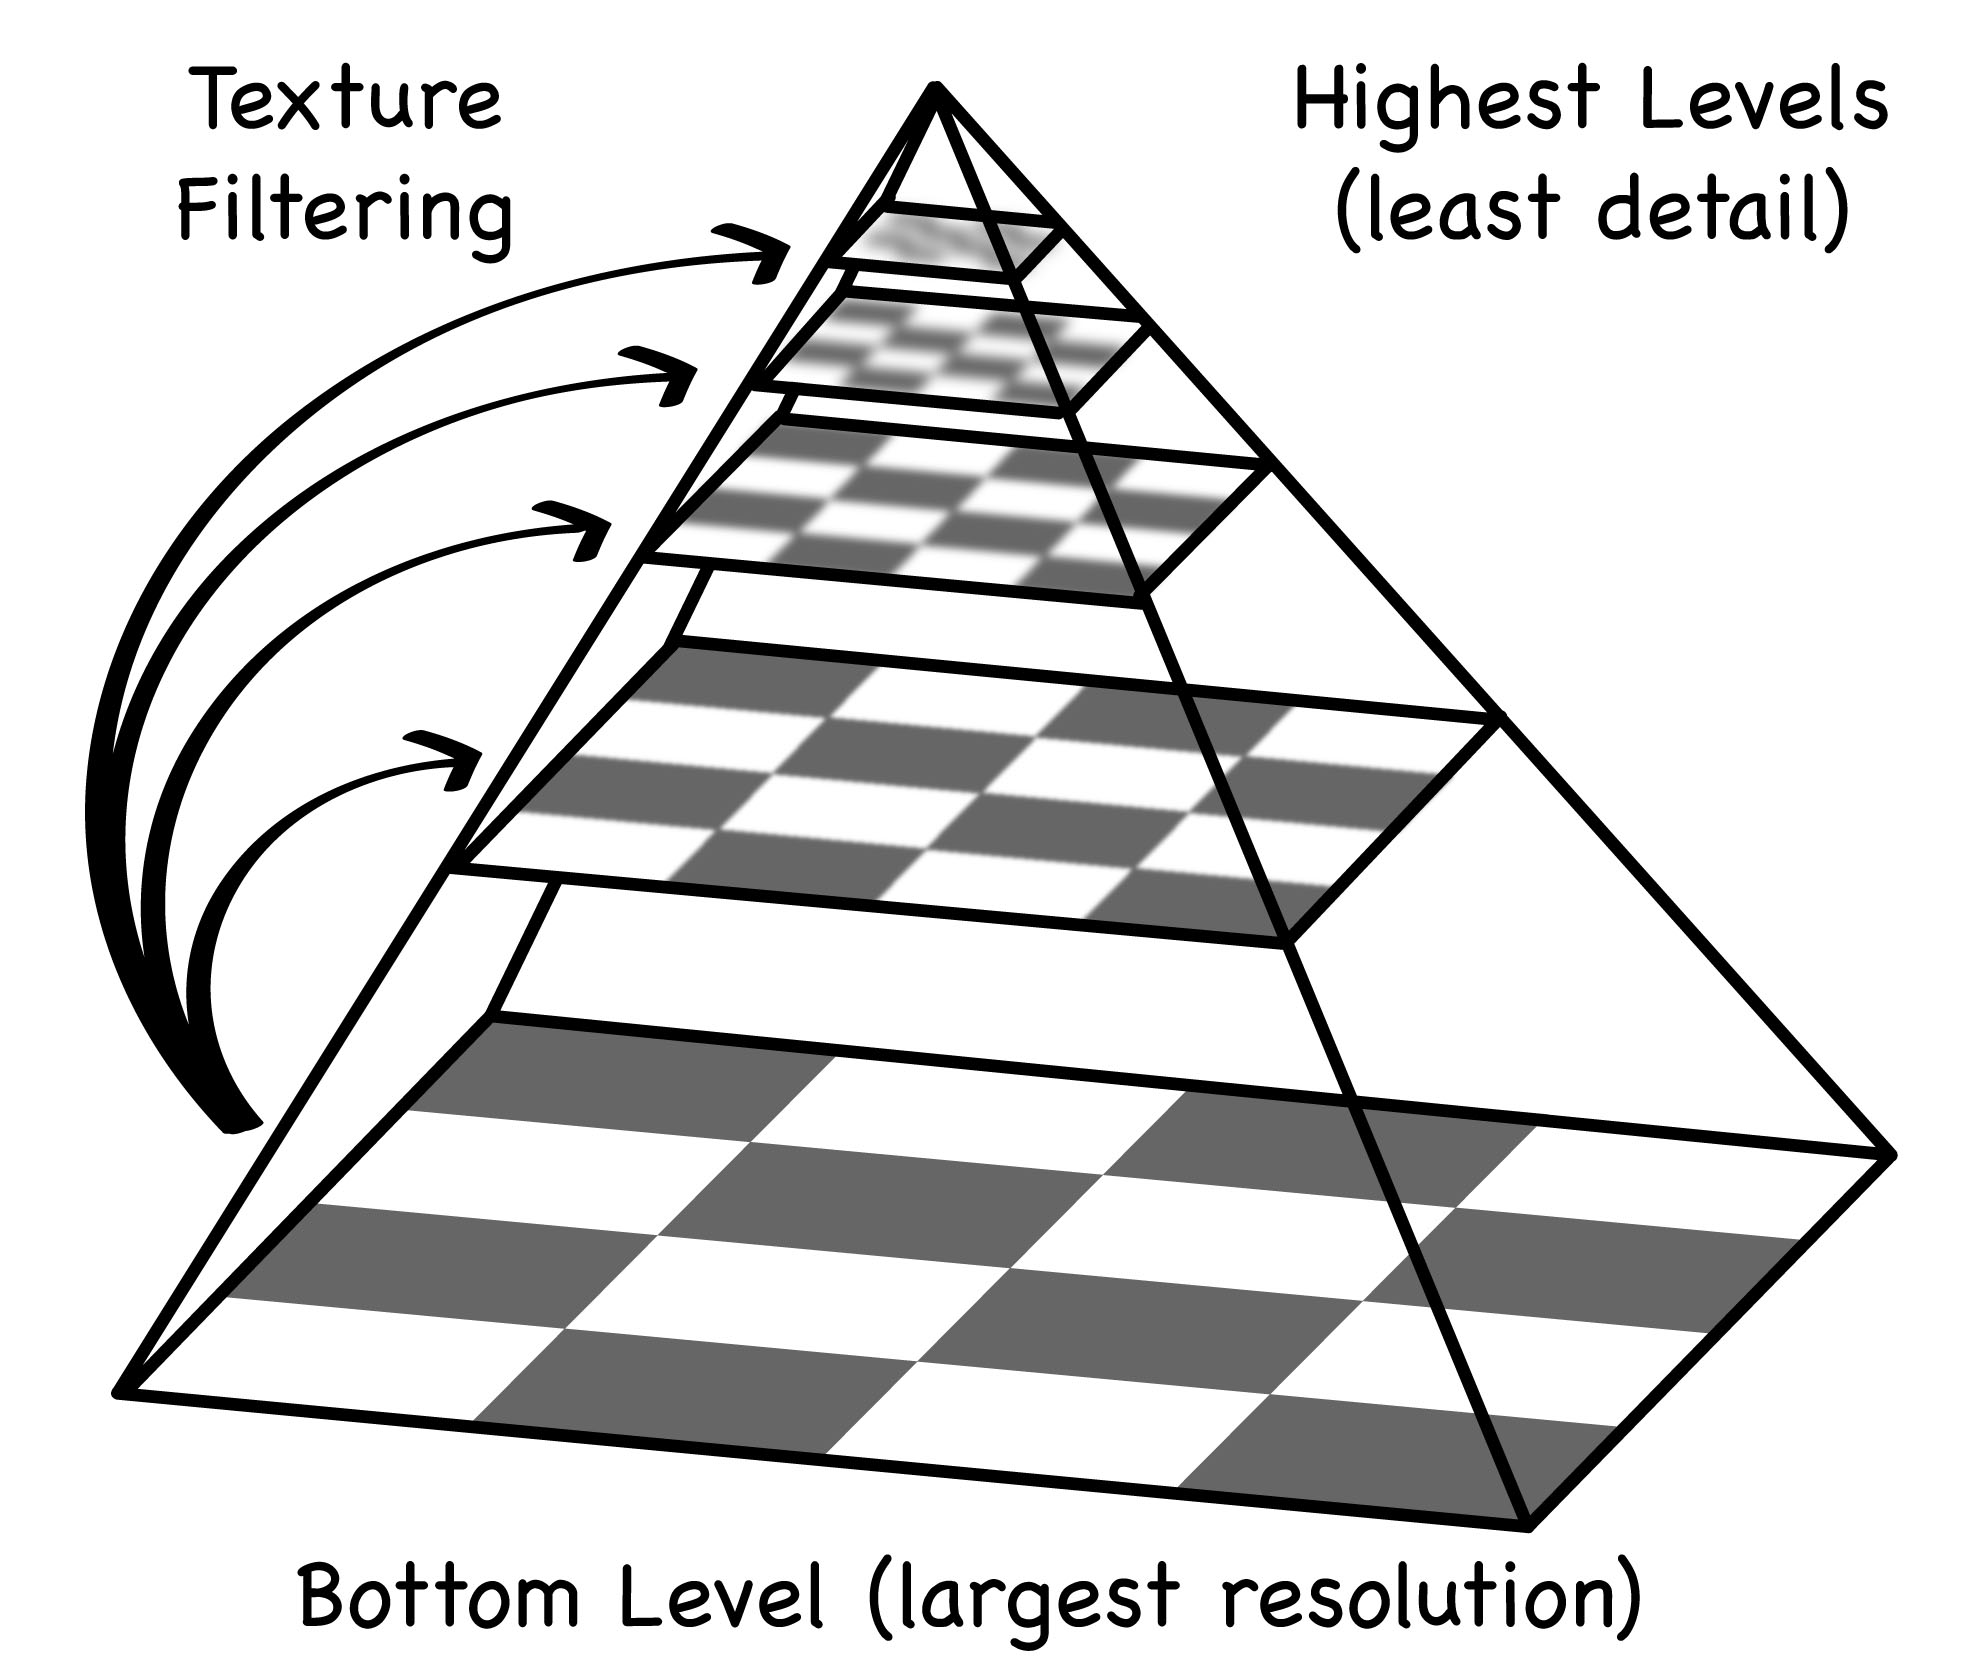
\includegraphics[width=0.5\linewidth]{2a.jpg}
  \label{fig2}
  \caption{Laplacial pyramid decomposition level}
\end{figure}

\section{Wavelet Transformation}
I start this section by introducing the specific concepts related to the wavelet transform, so that the reader
can understand the basic concepts associated with this transform. \hfill \break

 The analysis and synthesis procedures lead to the
pyramid-structured wavelet decomposition \cite{9}.The 1-D multiresolution wavelet decomposition can be easily extended to two dimensions by introducing separable 2-D scaling and wavelet functions as the tensor products of their 1-D complements. Hence, we obtain

\begin{equation}
    \begin{split}
    {\phi }_{LL}\left(x,y \right)=\phi \left(x \right)\phi \left(y \right)\vspace{1cm}
    {\psi }_{LH}\left(x,y \right)=\phi \left(x \right)\psi  \left(y \right)\\
	{\psi }_{HL}\left(x,y \right)=\psi \left(x \right)\phi  \left(y \right),\vspace{1cm}
	{\psi }_{HH}\left(x,y \right)=\psi \left(x \right)\psi  \left(y \right)  
    \end{split}
\end{equation}

The 2-D wavelet analysis operation consists in =ltering and
down-sampling horizontally using the 1-D lowpass =lterL(with impulse responses l(i)) and highpass =lterH(withimpulse responses h(j)) to each row in the imageI(x; y),producing the coeIcient matrices IL(x; y) and IH(x; y).
Vertically =ltering and down-sampling follows, using the lowpass and highpass =lters LandHto each column in IL(x; y) andIH(x; y) and produces four subimagesILL(x; y),ILH(x; y), IHL(x; y) and IHH(x; y) for one level of decomposition.ILL(x; y) is a smooth subimage corresponding to the low-frequency band of the MSD and can be considered as a smoothed and subsampled version of the original imageI(x; y), i.e. it represents the coarse approximation of I(x; y).ILH(x; y),IHL(x; y) andIHH(x; y) are detail subimages, which represent the horizontal, vertical and diagonal
directions of the imageI(x; y).
\begin{figure}[h]
  \centering
  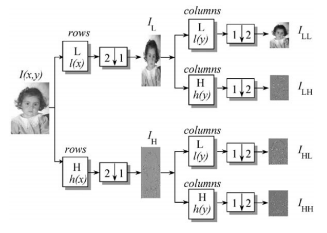
\includegraphics[width=0.5\linewidth]{2b.png}
  \label{fig2}
  \caption{ One stage of 2-D DWT multiresolution image decomposition
(forward wavelet analysis).}
\end{figure}

Fig \ref{fig2.2} depicts one stage in a multiresolution pyramid decomposition of the input imageI(x; y). In order to illustrate the
examples of this section, we have used the Haar wavelet
transform, although any other set of wavelets could be used.
Hence,L≡(1=√2)[1;1] and H≡(1=√2)[1;−1].The detailed 2-D pyramid decomposition algorithm, can be expressed as follows: Let I(x; y) be the original image of size M×N, l(i) the analysis lowpass coefficients of a specific wavelet basis, i =0;1,2......Nh−1, where Nl is the support length of the filter L, h(j) the analysis high pass coefficients of a specific wavelet basis,j=0,1....Nh−1, where Nh is the support length of the filter H. Then,

\begin{equation}
    \begin{split}
     {I}_{L}\left(x,y \right) &=\frac{1}{{N}_{l}} \sum_{i=0}^{{N}_{l}-1} I\left(i \right). I\left(\left(2x+i \right)modM,y \right),{I}_{H}\left(x,y \right)\\ &=\frac{1}{{N}_{h}} \sum_{j=0}^{{N}_{h}-1} h\left(j \right). I\left(\left(2x+j \right)modM,y \right) 
    \end{split}
\end{equation}
for x=0,1,2......M/2−1 and y=0,1,2......N−1

\begin{equation}
    \begin{split}
     {I}_{LL}\left(x,y \right) &=\frac{1}{{N}_{l}} \sum_{i=0}^{{N}_{l}-1} I\left(i \right). I\left(x,\left(2x+i \right)mod N \right),{I}_{LH}\left(x,y \right)
\\ &=\frac{1}{{N}_{h}} \sum_{j=0}^{{N}_{h}-1} h\left(j \right). I\left(x,\left(2y+j \right)mod N \right) 
    \end{split}
\end{equation}

\begin{equation}
    \begin{split}
    {I}_{HL}\left(x,y \right) &=\frac{1}{{N}_{l}} \sum_{i=0}^{{N}_{l}-1} I\left(i \right). {I}_{H}\left(x,\left(2y+i \right)mod N \right),{I}_{HH}\left(x,y \right) \\
\\ &=\frac{1}{{N}_{h}} \sum_{j=0}^{{N}_{h}-1} h\left(j \right). {I}_{H}\left(x,\left(2y+j \right)mod N \right)
    \end{split}
\end{equation}
for x=0,1,2......m/2-1 and y=0,1,2.....N/2-1 \\

The 2-D pyramid algorithm can iterate on the smooth subimage 
\({I}_{LL}\left(x,y \right)\) to obtain four coefficient matrices in the next decomposition level and so on. This is illustrated in Figs.\ref{fig2.3} and  which correspond to one-and two-level image decompositions, respectively.  \\ 

\begin{figure}[h]
  \centering
  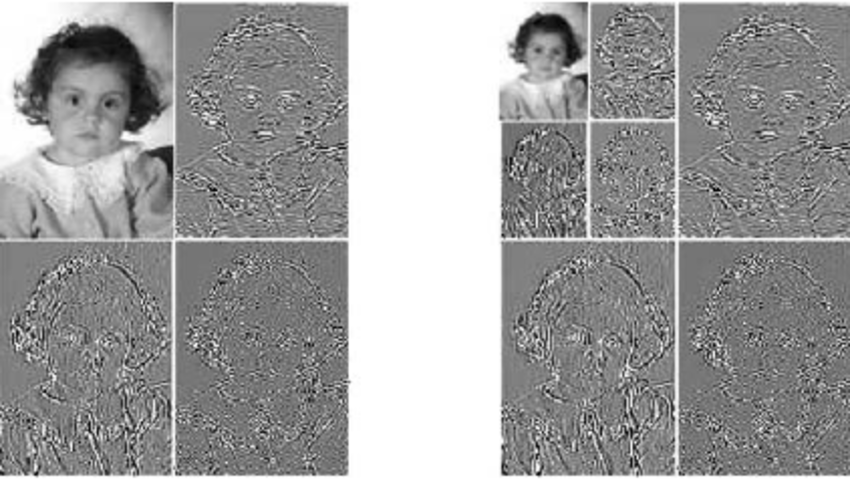
\includegraphics[width=0.5\linewidth]{2d.png}
  \label{fig2}
  \caption{ A representation of (a) one-level and (b) two-level image
decomposition.}
\end{figure}

Some wavelet-based applications do not require all coefficients, only the most relevant. So an additional procedure can be carried out to eliminate non-significant coefficient by thresholding, since these have a magnitude close to zero. After thresholding, only the desired coefficients remain.The threshold value can be chosen as \(T=\sigma\sqrt{2\log n/ \sqrt{n}}  \) in  where \(\sigma\)  is the standard deviation of the coefficients and n is the total size of samples. Another possibility is to fix T in order to replace a percentage of the coefficients with the
smallest magnitude to zero. Obviously, the cancellation of coefficients implies a loss of information. \\

The inverse 2-D wavelet transform can be implemented using a backward 2-D pyramid algorithm. The 2-D wavelet synthesis operation consists in up-sampling and filtering vertically using the 1-D synthesis lowpass filter
L(with impulse responses l(i)) and highpass filter H(with impulse
responses  h(j)) for each column in the subimage. Horizontal up-sampling and =ltering then follows, using the lowpass  Land highpass filter H, for each row of the reversed image. Fig. \ref{fig2.4} shows one stage in a wavelet reconstruction


\begin{figure}[h]
  \centering
  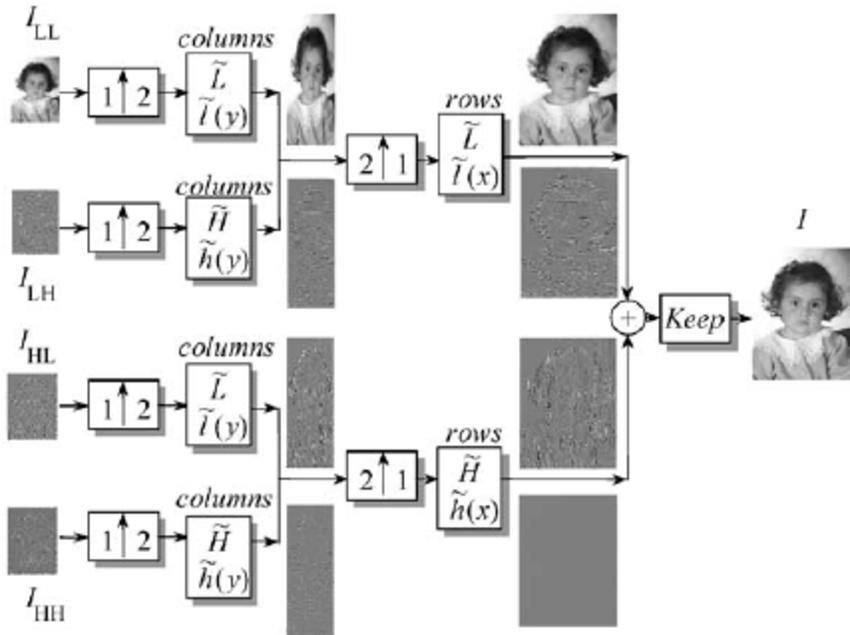
\includegraphics[width=0.5\linewidth]{2c.png}
  \label{fig2}
  \caption{One stage of 2-D DWT multiresolution image reconstruction
(backward wavelet synthesis).}
\end{figure}

\section{Fast Discrete Curvelet Transforms}
Despite considerable success, intense research in the last few years has shown that classical multiresolution ideas are far from being universally effective. Indeed, just as people recognized that
Fourier methods were not good for all purposes and consequently introduced new systems such as wavelets researchers have sought alternatives to wavelet analysis. In signal processing for example, one has to deal with the fact that interesting phenomena occur along curves or sheets, e.g.
edges in a two-dimensional image. While wavelets are certainly suitable for dealing with objects where the interesting phenomena, e.g. singularities, are associated with exceptional points, they
are ill-suited for detecting, organizing, or providing a compact representation of intermediate dimensional structures. Given the significance of such intermediate dimensional phenomena, there
has been a vigorous research effort to provide better adapted alternatives by combining ideas from geometry with ideas from traditional multiscale analysis 
\subsection{Why a discrete curvelet transform?}
Curvelets are interesting because they efficiently address very important problems where wavelet ideas are far from ideal. I give three examples:

\begin{itemize}
  \item Optimally sparse representation of objects with edges. Curvelets provide optimally sparse representations of objects which display curve-punctuated smoothness except for discontinuity along a general curve with bounded curvature. Such representations are nearly as sparse as if the object were not singular and turn out to be far more sparse than
the wavelet decomposition of the object.
  \item Optimally sparse representation of wave propagators. Curvelets may also be a very significant tool for the analysis and the computation of partial differential equations. For example, a remarkable property is that curvelets faithfully model the geometry of wave propagation. Indeed, the action of the wave-group on a curvelet is well approximated by simply translating the center of the curvelet along the Hamiltonian flows. A physical interpretation of this result is that curvelets may be viewed as coherent waveforms with enough frequency localization so that they behave like waves but at the same time, with enough spatial localization so that
they simultaneously behave like particles 
  \item Optimal image reconstruction in severely ill-posed problems. Curvelets also have special micro local features which make them especially adapted to certain reconstruction problems with missing data.
\end{itemize}

\subsection{Digital Curvelet Transform via Wrapping} 
The ‘wrapping’ approach assumes the same digital coronization as in Section 3.1, but makes a different, somewhat simpler choice of spatial grid to translate curvelets at each scale and angle. Instead of a tilted grid, we assume a regular rectangular grid and define ‘Cartesian’ curvelets in essentially the same way as before,
\begin{equation} \label{eq:2.5}
 c\left(j,l,k \right)=\int \hat{f}\left(\omega  \right){U}_{j}\left({S}^{-1}\omega  \right){e}_{i<b\omega> }
\end{equation}
The difficulty behind this approach is that, in the frequency plane, the window \({U}_{j,l}\left[n1,n2 \right] \) does not
fit in a rectangle of size \({2}^{j} {2}^{j/2}  \), aligned with the axes, in which the 2D IFFT could be applied to compute \ref{eq:2.5}. After discretization, the integral over \(\omega \) becomes a sum over n1, n2 which would extend beyond the bounds allowed by the 2-D IFFT. The resemblance of \ref{eq:2.5} with a standard 2D inverse FFT is in that respect only formal.hanged.\\

To understand why respecting rectangle sizes is a concern, we recall that \({U}_{j,l}\)  is supported in the parallelepipedal region
    
 \subsection{Architecture of the FDCT}   
 
 \begin{itemize}
  \item Apply the 2D FFT and obtain Fourier samples \( \hat{f}\left[n1,n2 \right],-n/2 \leq n1,n2 \leq n/2   \)
  \item  For each scale j and angle, form the product \({U}_{j,l} \hat{f}\left[n1,n2\right] \)
  \item  Wrap this product around the origin and obtain
  \item  Apply the inverse 2D FFT to each \({f}_{j,l} \), hence collecting the discrete coefficients \({c}^{D} \left(j,l,k\right) \)
\end{itemize}